\section{L06-Sistemi aperti}
\subsection{Sistema aperto}
\begin{center}
    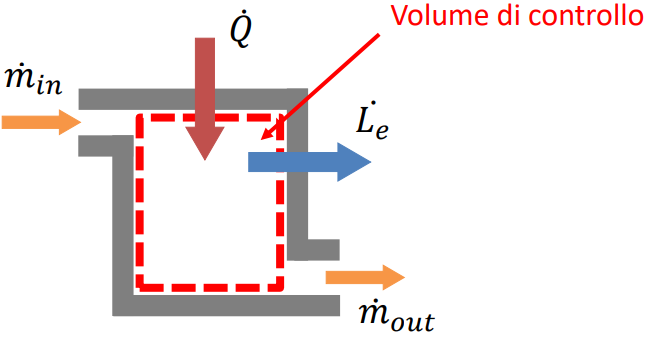
\includegraphics[height=3cm]{../L06/img1.PNG}
\end{center}
Un \textbf{sistema aperto} è un sistema dal quale può \textbf{uscire} ed \textbf{entrare massa}, per semplicità consideriamo una sola sezione di ingresso ed una sola sezione di uscita.\newline
\newline
Il sistema è percorso da \textbf{flussi monodimenisonali}:
\begin{itemize}
    \item sono presenti \textbf{condizioni di equilibrio} termodinamico sulle sezioni di \textbf{ingresso} e di \textbf{uscita};
    \item non viene fatta alcuna ipotesi in merito alla trasformazione termodinamica che il fluido subisce all'interno del sistema;
\end{itemize}
\ \newline
E' un \textbf{sistema fluente} e di conseguenza è necessario introdurre la \textbf{variabile tempo} ($t$) e di conseguenza i \textbf{flussi di massa}, \textbf{di energia}, \textbf{di entropia}, etc.
\[
    \dot{m} \;\;\;\;\; \dot{E}\;\;\;\;\;\dot{U}\;\;\;\;\;\dot{H}\;\;\;\;\;\dot{S}\;\;\;\;\;\dot{Q}\;\;\;\;\;\dot{L}
\]
\subsection{Equazioni di bilancio}
\subsubsection{Bilancio di massa}
Il bilancio di massa analizza la variazione di massa nel tempo del volume di controllo.
\[
    \frac{dM}{dt} = \sum_{k} \dot{m}_k^\leftarrow
\]
dove per $k$ si intendono le sezioni di passaggio, nel nostro caso 2, quella d'ingresso e quella d'uscita:
\[
    \frac{dM}{dt} = \dot{m}_i - \dot{m}_u
\]
\textbf{Equazione di continuità}:
\[
    \dot{m}=\rho w \Omega
\]
$\dot{m}$: portata;\newline
$\rho$: massa volumica;\newline
$w$: velocità media;\newline
$\Omega$: area della sezione di passaggio;
\subsubsection{Bilancio di energia}
\[
    \frac{dE}{dt}=\dot{E}^\leftarrow 
\]
L'\textbf{energia netta} entrante nel sistema:
\[
    \dot{E}^\leftarrow = \dot{Q}^\leftarrow - \dot{L}^\rightarrow + \sum_{k}\dot{E}_{m,k}^\leftarrow  + sorgenti
\]
$\dot{Q}^\leftarrow $: calore scambiato;\newline
$\dot{L}^\rightarrow $: lavoro scambiato;\newline
La sommatoria rappresenta lo scambio di energia associata al trasporto di massa per ogni sessione di passaggio, nel nostro caso 2, quelal d'ingresso e quella d'uscita;\newline
Le sorgenti sono le fonti di energia dovute a sorgenti (es. radiazioni, reazioni chimiche, etc.).\newline
\subsubsection{Calore scambiato}
\begin{itemize}
    \item Calore scambiato per unità di tempo attraverso le sezioni non attraversate dalla massa: $\dot{Q}^\leftarrow $;
    \item Calore scambiato per unità di tempo attraverso le sezioni attraversate dalla massa (ingresso e uscita): \textbf{trascurabile}
\end{itemize}
\subsubsection{Lavoro scambiato}
\begin{itemize}
    \item Lavoro scambiato per unità di tempo attraverso le sezioni non attraversate dalla massa: \textbf{lavoro di elica} $-\dot{L}_e^\rightarrow $ (che è la potenza meccanica che possiamo sfruttare);
    \item Lavoro scambiato per unità di tempo attraverso le sezioni attraversare dalla massa (ingresso e uscita): \textbf{lavoro di pulsione} $\dot{L}_P^\leftarrow $
\end{itemize}
\subsubsection{Lavoro di pulsione}
il \textbf{lavoro di pulsione} è il lavoro necessario per immettere nel sistema la massa che il sistema scambia con l'esterno.
\begin{center}
    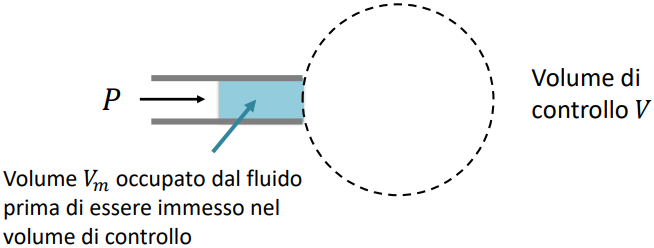
\includegraphics[height=3cm]{../L06/img2.PNG}
\end{center}
Si consideri un sistema $V + V_m$ occupato dalla massa $M + M_i$. Se si immette la massa $M_i$ nel volume $V$ il sistema complessivo subisce una variazione (riduzione) di volume mantenendo costante la massa.\newline
\newline
Questo è un sistema chiuso che scambia con l'esterno un lavoro $L_P^\leftarrow $:
\[
    L_P^\leftarrow  = - \int_{V-V_m}^{V}Pdv = P V_m
\]
dove $P$ è una costante. \newline
\newline
Per la \textbf{sessione di ingresso}:
\[
    L_P^\leftarrow  = M_i P v_i
\]
dove \newline
$M_i$: massa immessa nel sistema;\newline
$P$: pressione costante che agisce su $M_i$; \newline
$v_i$: volume specifico della sessione di ingresso.\newline
Allo stesso modo possiamo calcolarlo per la \textbf{sessione di uscita}.\newline
\newline
Questo termine di lavoro compare per ogni sezione di ingresso e di uscita della massa.
\subsubsection{Energia associata al trasporto di massa}
Nel valutare l'energia entrante nel sistema occorre tenere presente che la massa che attraversa la superficie di controllo trasporta con sè energia ($E_m$).\newline
\newline
Risulta somma delle energie associate ai flussi di massa (energia interna, energia potenziale ed energia cinetica):
\[
    \dot{E}_m = \sum_{k} \dot{m}_k^\leftarrow \left(u + gz + \frac{w^2}{2}\right)_k
\]
dove \newline
$k$: è il solito indice che itera su tutte le sessioni di scambio con l'esterno, nel nostro caso sono 2, quella di ingresso e quella d'uscita;\newline
$\dot{m}_k^\leftarrow $: portata; \newline
$u$: energia interna;\newline
$gz$: energia potenziale, con $g$ accellerazione gravitazionale e $z$ altitudine della sessione di passaggio;\newline
$\frac{w^2}{2}$: velocità media.
\subsubsection{Bilancio energetico}
Ritorniamo ora sul bilancio di energia 
\[
    \frac{dE}{dt} = \dot{E}_m + \dot{Q}^\leftarrow - \dot{L}_e^\rightarrow + \sum_{k}(\dot{L}_P^\leftarrow)_k
\]
ma espandiamo tutti i termini che abbiamo visto:
\[
    \frac{dE}{dt} = \dot{m}_i \left( u + gz + \frac{w^2}{2} \right)_i - \dot{m}_u \left( u + gz + \frac{w^2}{2} \right)_u + \dot{Q}^\leftarrow - \dot{L}_e^\rightarrow  + \dot{m}_i(Pv)_i - \dot{m}_u(Pv)_u
\]
dove \newline
$\dot{m}_i \left( u + gz + \frac{w^2}{2} \right)_i$ è l'energia associata alla massa entrante.\newline
$\dot{m}_u \left( u + gz + \frac{w^2}{2} \right)_u$ è l'energia associata alla massa uscente. \newline
$\dot{Q}^\leftarrow$  è il valore entrante dal contorno del sistema.\newline
$\dot{L}_e^\rightarrow$ è il lavoro uscente dal contorno del sistema (di elica).\newline
$\dot{m}_i(Pv)_i$ è il lavoro di pulsione all'ingresso.\newline
$\dot{m}_u(Pv)_u$ è il lavoro di pulsione all'uscita.\newline
\newline
Ricordando ora che l'entalpia di una sessione generica $k$ è esprimibile come $(u +Pv)_k = (h)_k$ possiamo riscrivere l'espressione come:
\[
    \frac{dE}{dt} = \sum_{k}\dot{m}_k^\leftarrow  \left( h + gz + \frac{w^2}{2} \right)_k + \dot{Q}^\leftarrow  - \dot{L}_e^\rightarrow 
\]
\subsubsection{Bilancio entropico}
In modo analogo al bilancio di energia è possibile ricavare l'equazione di bilancio entropico:
\[
    \frac{dS}{dt} = \sum_{k} \dot{m}_k^\leftarrow s_k + \dot{S}_Q^\leftarrow  + \dot{S}_{irr}
\]
\subsubsection{Regime stazionario}
Tra le situazioni che si presentano più frequentemente in ingegneria vi sono le cosiddette \textbf{condizioni di stazionarietà o di regime permanente}, in cui le variazioni di massa, di energia e di entropia nel sistema sono nulle nel tempo:
\[
    \frac{dM}{dt} = 0 \;\;\;\;\;\;\;\;\;\;\frac{dE}{dt} = 0 \;\;\;\;\;\;\;\;\;\;\frac{dS}{dt} = 0
\]
Con questa semplificazione i bilanci visti precedentemente diventano:
\[
    \dot{m}_i^\leftarrow  = - \dot{m}_u^\leftarrow  = \dot{m}
\]
\[
    \dot{m}\left[(h_i-h_u) + g (z_i-z_u) + \frac{w_1^2 - w_u^2}{2}\right] + \dot{Q}^\leftarrow  - \dot{L}_e^\rightarrow  = 0
\]
\[
    \dot{m}(s_i - s_u) + \dot{S}_Q^\leftarrow  + \dot{S}_{irr} = 0
\]
\subsection{Macchina aperta}
La \textbf{macchina aperta} è un \textbf{dispositivo adiabatico} destinato a \textbf{scambiare lavoro} per il quale si ipotizzano trascurabili le variazioni di energia potenziale e di energia cinetica tra le sezion idi ingresso e di uscita.\newline
\newline
I bilanci diventano:
\[
    \dot{m}(h_i - h_u) - \dot{L}_e^\rightarrow  = 0 \;\;\;\;\;\;\;\;\;\;\;\;\;\;\; \dot{m} (s_i - s_u) + \dot{S}_{irr} = 0
\]
\textbf{Turbina}:
\begin{center}
    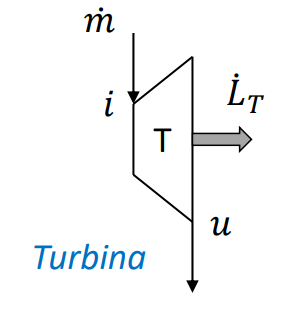
\includegraphics[height=4cm]{../L06/img3.PNG}
\end{center}
La macchina termica prende il nome di turbina se produce lavoro, cioè genera potenza meccanica. Le turbine sfruttano il flusso di massa al loro interno per trasformare l'energia che la massa porta in lavoro da scambiare con l'esterno. Come lo fanno? la turbina ottiene il suo scopo riducendo il suo contenuto entalpico. Se parliamo di un gas in una turbina, quest'ultimo si espande, riduce la sua pressione e temperatura, e così aumenta il suo volume specifico. Da notare che nel disegno il lato di ingresso è quello corto e quello d'uscita è quello lungo, per simboleggiare che la sostanza si espande. nel caso della turbina il lavoro di elica uscente è positivo, quindi l'entalpia in ingresso è maggiore dell'entalpia in uscita.\newline
\newline
\textbf{Compressore e pompa}:
\begin{center}
    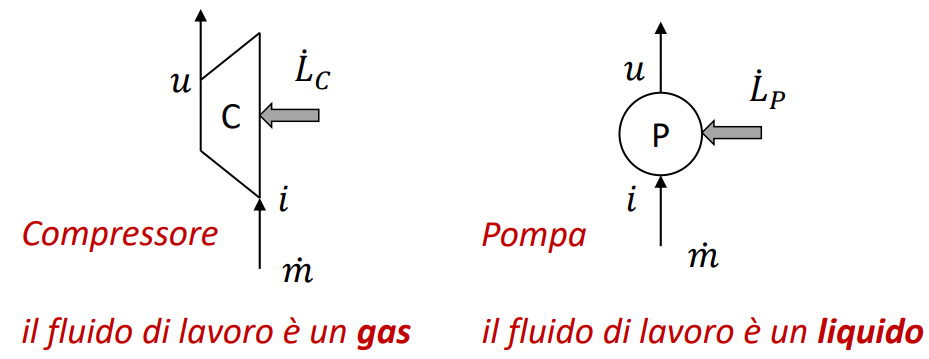
\includegraphics[height=4cm]{../L06/img4.PNG}
\end{center}
Se la macchina aperta ssorbe lavoro dall'esterno, si parla di compressore o pompa a seconda del fluido di lavoro. Nel compressore la situazione è opposta a quella della turbina: la potenza meccanica inserita nel compressore è trasformata in entalpia. La pompa cerca di aumentare la pressione del liquido al suo interno, la differenza col compressore sta nel fatto che essendo il liquido solitamente incomprimibile, il volume specifico del liquido non varia.
\subsection{Scambiatore di calore}
Lo \textbf{scambiatore di calore} è un dispositivo destinato a \textbf{scambiare calore} e che \textbf{non scambia lavoro} per il quale si ipotizzano trascurabili le variazioni di enregia potenziale e di energia cinetica tra le sezioni di ingresso e di uscita.\newline
E' la macchina opposta alla macchina aperta.\newline
Lo scambio di calore può essere entrante o uscente.
\begin{center}
    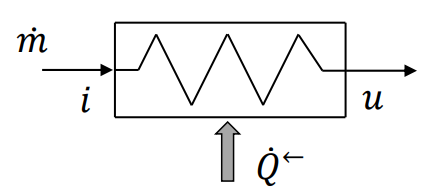
\includegraphics[height=3cm]{../L06/img5.PNG}
\end{center}
I bilanci diventano:
\[
    \dot{m} (h_i - h_u) + \dot{Q}^\leftarrow  = 0 \;\;\;\;\;\;\;\;\;\;\;\;\;\;\;\dot{m} (s_i -s_u) + \dot{S}_Q^\leftarrow  + \dot{S}_{irr} = 0
\]
\subsection{Diffusore e ugello}
I \textbf{diffusori} ($w \searrow$) e gli \textbf{ugelli} ($w \nearrow$) sono sistemi aperti stazionari che operano \textbf{senza scambio di lavoro nè calore} per i quali si ipotizzano trascurabili le variazioni di energia potenziale tra le sezioni di ingresso e di uscita.\newline
La differenza fra diffusore e ugello dipende se lo stato di ingresso si trova a una velocità di ingrsso maggiore (diffusore) rispetto a quella d'uscita o viceversa (ugello).
\begin{center}
    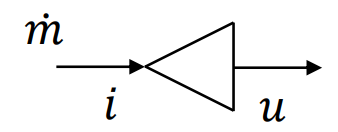
\includegraphics[height=3cm]{../L06/img6.PNG}
\end{center}
I bilanci diventano:
\[
    \left[(h_i - h_u) + \frac{w_i^2 - w_u^2}{2}\right] = 0
\]
\[
    \dot{m} (s_i - s_u) + \dot{S}_{irr} = 0
\]
\subsection{Valvola di laminazione}
La \textbf{valvola di laminazione} è un \textbf{dispositivo adiabatico} che \textbf{non scambia lavoro} per il quale si ipotizzano trascurabili le variazioni di energia potenziale e di energia cinetica tra le sezioni di ingresso e di uscita. Si ottiene un processo detto di \textbf{laminazione isoentalpica} (cioè in cui l'entalpia in ingresso e in uscita sono identiche).\newline
A livello pratico ciò che succede in questo sistema è che la pressione scende fra ingresso e uscita (come se ci fosse uno strozzamente).
\begin{center}
    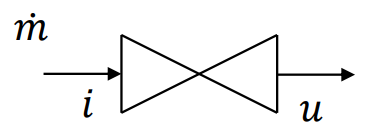
\includegraphics[height=3cm]{../L06/img7.PNG}
\end{center}
I bilanci diventano:
\[
    (h_i-h_u) = 0 \;\;\;\;\;\;\;\;\;\;\;\;\;\;\;\dot{m}(s_i - s_u) + \dot{S}_{irr} = 0
\]
Da notare che il processo è \textbf{irreversibile} ed è presente la componente $\dot{S}_{irr}$.
\subsection{Rendimento isoentropico di una macchina aperta}
\subsubsection{Turbina}
Si chiama \textbf{rendimento isoentropico} di una \textbf{macchina motrice aperta} (turbina) il rapporto fra la potenza realmente ottenuta e la potenza massima ottenibile in condizioni ideali (trasformazione del fluido isoentropica e quindi adiabatica reversibile) a parità di condizioni in ingresso e a partià di pressione di fine espansione.
\[
    \eta_T = \frac{\dot{L}_{reale}^\rightarrow}{\dot{L}_{ideale}^\rightarrow } = \frac{(h_1-h_{2'})}{(h_1-h_2)}
\]
\begin{center}
    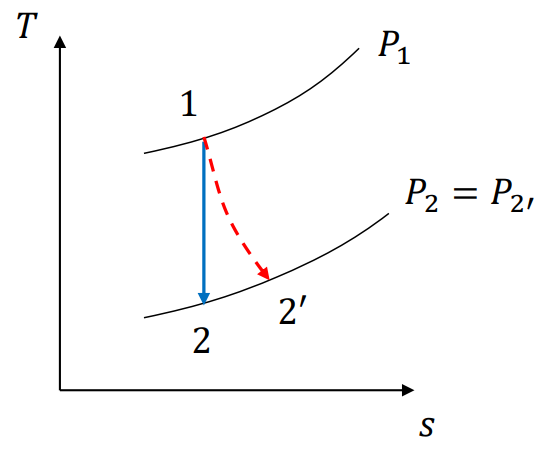
\includegraphics[height=4cm]{../L06/img8.PNG}
\end{center}
Per esempio un produttore di turbine, calcolare quale sarebbe la potenza meccanica prodotta in modo ideale con uan certa pressione (e temperatura) di ingresso (1) e una certa pressione (e temperatura) di uscita (2), poi nella realtà si va a misurare i valori efferrivamente trovati (2'). Andando a confrontare i deu valori delle due potenze emccaniche calcolare (quella della turbina ideale e quella della turbina reale) possiamo trovare il parametro del rendimento isoentropico. Questo parametro mostra le prestazioni della turbina.
\subsubsection{Compressore e pompa}
Si chiama \textbf{rendimento isoentropico} di una \textbf{macchina operatrice aperta} (compressore e pompa) il rapporto fra la potenza minima spesa in condizioni ideali (trasformazione del fluido isoentropica e quindi adiabatica reversibile) e la potenza realmente spesa a parità di condizioni in ingresso e a parità di pressione di fine espansione.
\[
    \eta_C =  \frac{\dot{L}_{reale}^\rightarrow}{\dot{L}_{ideale}^\rightarrow } = \frac{(h_1-h_2)}{(h_1-h_{2'})}
\]
\begin{center}
    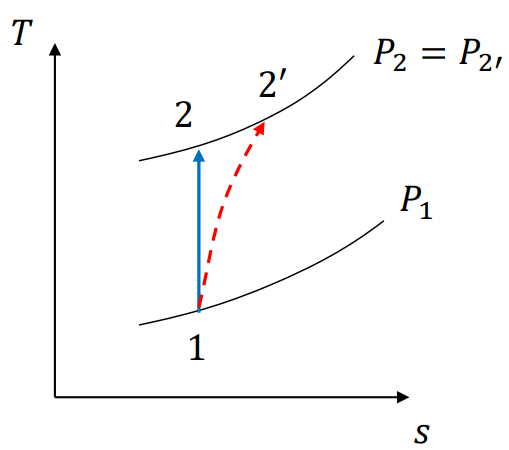
\includegraphics[height=4cm]{../L06/img9.PNG}
\end{center}
\subsection{Irreversibilità interna e lavoro specifico}
Illustrazione e dimostrazione del legame fra le irreversibilità che possono accadere all'interno di un sistema aperto e altre grandezze (in questo caso la temperatura). Vediamo una dimostrazione:
\subsubsection{Irreversibilità interna associata al moto del fluido}
Si consideri il moto stazionario di un fluido in un tratto di condotta infinitesimo con l'ipotesi che lo scambio di calore con l'esterno sia realizzato in modo reversibile. Dopo opportuni passaggi e trascurando le variazioni di energia cinetica e potenziale, il bilancio energetico ed entropico per unità di massa sono:
\[
    -dh +\delta q_{rev}^\leftarrow  - \delta l_{e}^\rightarrow  = 0
\]
\[
    - ds + \frac{\delta q_{rev}^\leftarrow }{T} + d s_{irr} = 0
\]
e quindi
\[
    Tds = \delta q_{rev}^\leftarrow  + Tds_{irr}
\]
Ricordando che $dh = du + vdP + Pdv$ (definizione) e $du = \delta q^\leftarrow  - \delta l^\rightarrow $ (primo principio), essendo $u$ funzione di stato posso considerare una trasformazione reversibile e scrivere $du = Tds - Pdv$, da cui otteniamo $d0 = Tds + vdP$.\newline
Si ottiene quindi
\[
    dh = \delta q_{rev}^\leftarrow  - \delta l_{e}^\rightarrow 
\]
\[
    dh = \delta q_{rev}^\leftarrow  + Tds_{irr} + vdP
\]
e quindi
\[
    \delta l_{e}^\rightarrow  = -vdP -Tds_{irr}
\]
Integrando fra la sezione di ingresso e quella di uscita:
\[
    l_e^\rightarrow  = - \int_{i}^{u} vdP - \int_{i}^{u}Tds_{irr}
\]
dove \newline
$\int_{i}^{u} vdP$ è il lavoro reversibile di elica $l_{rev}^\rightarrow $ (da notare che nel sistema chiuso questo era uguale all'integrale di $Pdv$ e qua è diventato l'integrale di $vdP$!);\newline
$\int_{i}^{u}Tds_{irr}$ è l'energia dissipata per irreversibilità interna (in generale porta a un incremento di $T$).\newline
\newline
Cosa ne deduciamo?\newline
Per esempio in una turbina il lavoro d'elica è positivo ed essendo la temperatura e $s_{irr}$ positivi, ottengo che se ho irreversibilità il mio lavoro è minore rispetto al lavoro reversibile, perchè uan parte della mia energia viene dissipata per via delle irreversibilità interne (es. gli attriti), in generale questo comporta un aumento della temperatura.\newline
Nell'esempio del compressore, invece, il lavoro d'elica è negativo (spendiam oenergia per far funzionare il compressore) e qunado ci sono irreversibilità ho una spesa maggiore rispetto al caso ideale, perchè una parte dell'energia viene dissipata dalle irreversibilità interne, quindi anche qua c'è spesso un inremento di temperatura.\newline
\newline
In generale l'irreversibiltà interna associata al moto di traduce in una spesa energetica per movimentare il fluido che però essere espressa come
\[
    \dot{L} = \dot{V} \Delta P
\]
dove \newline
$\dot{L}$: potenza meccanica necessaria a movimentare il fluido ($W$);\newline
$\dot{V} = w \Omega$: portata volumetrica ($m^3/s$); \newline
$\Delta P$: perdite di carico (Pa), questa variazione di pressione dipende dal fluido, dalle condizioni della macchina e da molti altri fattori come attrito, cambi di direzione, cambi di sezione, ostacoli, etc. Le perdite di carico sono la differenza che c'è fra il comportamento ideale e quello reale, le perdite di carico sono la componenete legata alle irreversibilità del sistema.\newline
\newline
Nel caso di \textbf{perdite di carico concentrate}:
\[
    \Delta P = K \rho \frac{w^2}{2}
\]
con pressione dinamica $\rho \frac{w^2}{2}$ e la costante di proporzionalità $K$ che dipende dalla singolarità geometrica e che è determinata sperimentalmente. QUalche esempio nella seguente tabella:
\begin{center}
    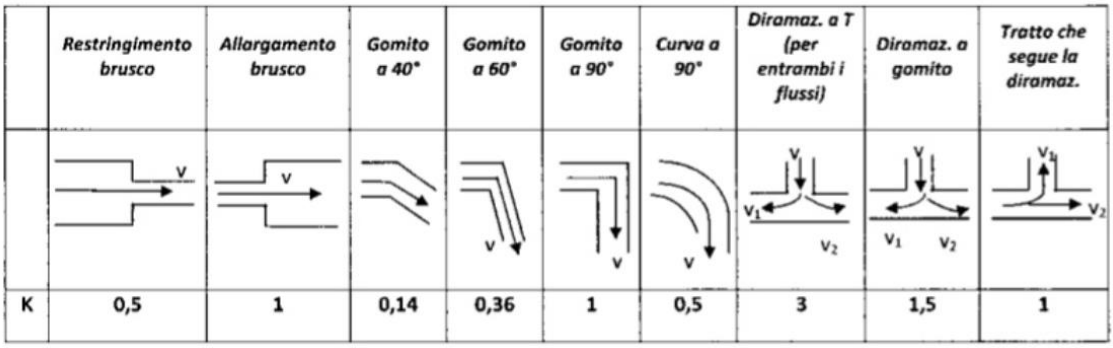
\includegraphics[height=3cm]{../L06/img10.PNG}
\end{center}
\ \newline
Nel caso di \textbf{perdite distribuite} (energia dissipata per via dell'attrito):
\[
    \Delta P = f \frac{L}{D} \rho \frac{w^2}{2}
\]
con pressione dinamica $\rho \frac{w^2}{2}$ e con $L$ e $D$ rispettivamente la lunghezza ed il diametro del condotto. Il coefficiente adimensionale $f$ è detto fattore di attrito (di Darcy) ed è funzione delle caratteristiche di moto del fluido, in particolare del numero di Reynolds ($Re = \rho w D /\mu$).\newline
\newline
Per moto laminare ($Re < 2000$): $f = \frac{64}{Re}$\newline
Per un moto turbolento (Blausius): $f = \frac{0.3164}{Re^{0.25}}$